%------------------------------------------------------------------------- 
\Section{Architecture of the proposed system}
\label{sec:architecture}
The following diagram depicts the simplified version of J3 JVM with some of the important components which have been added and modified to perform our goal which is an adaptive approach during an execution of the program.  Currently J3 JVM including VMKit doesn't provide any adaptive mode of execution which is basically switching to different level of optimized code dynamically during a runtime.  Current implementation of the J3 directly absorbs user's Java byte code and converted into in intermediate form called LLVM IR and finally it is generated into machine code according to the platform which the program being executed. Once LLVM IR has emitted in to machine code VMKit doesn't have a direct control over the instruction being executed in the back-end architecture . Instead of Jitting all the functions in to machine code VMKit only compiles whenever functions are being invoked very first time. So, subsequent invocation of the compiled function will be fetched from memory rather than coming back to front end every time of the function calls.

\begin{figure}[ht!]
\centering
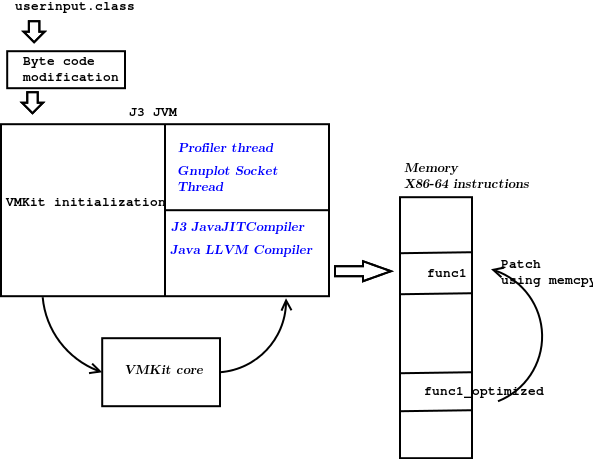
\includegraphics[width=80mm]{proposed_sytem.png}
\caption{Modified components in existing VMKit}
\label{fig:architecture}
\end{figure}

It would be more efficient if we could able to collect runtime information of each functions which are being executed in back-end and replace the most frequent function with the new level of optimization.  In order to achieve this goal and to demonstrate the adaptive approach in VMKit the following components have been added in to the existing VMKit implementation.

\Section{Byte code modification}
One of the basic information which has to be collected to perform function call frequency is obviously a number of time that particular function has been invoked. This will be achieved by hooking some byte code information in the given user's Java byte code. Every function in the Java byte code  will be modified with different unique global counters and extra functions also will be added to return the corresponding global counters.  The following Java snippet shows how given class file will be modified.

\tiny\begin{verbatim}
 public class Source
{
   public void calculateAnswer(int input)
     {
       int  result = input * 5;
     }
    public static void main(String[] args)
      {
          Source source = new Source();
          source.calculateAnswer(4);
      }

}
\end{verbatim}
\normalsize
\scriptsize{Above Java source file will be converted in to following format before we actually pass to J3 JVM}
\tiny\begin{verbatim}
public class Source
{
   private static int group2S_SourcecalculateAnswer=0;
   private static int group2E_SourcecalculateAnswer=0;
   public void calculateAnswer(int input)
     {
       ++group2S_SourcecalculateAnswer;
       int  result = input * 5;
       ++group2E_SourcecalculateAnswer;

     }
   int group2S_SourcecalculateAnswer()
     {
      return group2S_SourcecalculateAnswer;
     }

   int group2E_SourcecalculateAnswer()
     {
      return group2E_SourcecalculateAnswer;
     }

    public static void main(String[] args)
      {
          Source source = new Source();
          source.group2S_SourcecalculateAnswer();
          source.group2E_SourcecalculateAnswer();
          source.calculateAnswer(4);
      }


}
\end{verbatim}
\normalsize
Even though this modification will be taking place in the byte code level, actual source Java file and corresponding modified source has given here for reader's convenient.  The above actual source file has been modified by adding two global variable for each function which will to be used to achieve the following goals.


\begin{enumerate}
  \item Need to precisely identity whether the particular function is still spending time on a specific function block
  \item These two counters will be checked during the replacement of different level optimization
\end{enumerate}

Further, global variable return functions also will be added as shown in the modified Java file to let the J3 profiler thread to access the global counters in the specific interval. These global functions have forcefully been called by main method so that J3 knows where these global variables are being placed in the memory.

\subsection{LLVM-IR Optimization}
Optimizations are implemented as Passes that traverse some portion of a program to either collect information or transform the program.  Our implementation uses two different passes which are non optimized passes and full optimized passes. So, in the initial start up all the function will use the non optimized passes to generate the LLVM-IR and eventually fully optimized  passes will also apply to generate more optimized code. The following example function with some unused code shows the non optimized  LLVM IR.  Without any optimization passes huge LLVM IR will be generated as a result.  After the all passes most of the redundant code blocks have  eliminated  and as a result smaller machine code will be emitted.\\

\scriptsize\begin{verbatim}
public void Calc1() 
    { 
      ++group2S_GameCalc1
      double x=0.001; 
      for (int z = 0; z < 10000; z++) 
           {	 
              double a=2+x; 
              double b=x+a; 
              ouble c=x+b; 
              double d=x+c;
              double e=x+d; 
              x+=e; 
            } 
      ++group2E_GameCalc1;
    }

\end{verbatim}

\textbf{Unoptimized LLVM IR of Calc1 function}
\begin{verbatim}
; Function Attrs: noinline nounwind 
define void @32(%JavaObject*) #6 gc "vmkit" { 
   ---------------
   ---------------

"false IF_ICMPGE": ; preds = %afterSafePoint4 
  store double 2.000000e+00, double* %stack_double_0 
  store i32 0, i32* %stack_int_1 
  %33 = load double* %double_1 
  store double %33, double* %stack_double_2 
  store i32 0, i32* %stack_int_3 
  ----------------
  %84 = load i32* %stack_int_1 
  %85 = load double* %stack_double_0 
  store double %85, double* %double_1 
  %86 = load i32* %int_3 
  %87 = add i32 %86, 1 
  store i32 %87, i32* %int_3 
  br label %13 
} 

\end{verbatim}
\normalsize
The above IF\_ICMPGE will be completely removed during the optimization passes. 
\subsection{Profiler thread}

Once J3 JVM started up, Profiler thread also will be fired to keep evaluate the global counters of each functions which have been already been compiled in to machine code.  Each and every function will be concatenated with responsible class name to generate a key and value as a C structure which will be having the following fields. This profiler thread is fully responsible for monitoring function statistics , generating necessary information to calculate function call frequency and finally patching the optimized version of high frequency function.
\scriptsize\begin{verbatim}
      
typedef struct Patch {
        void *llvmGlobalVariableStartMachinePointer;
        void *llvmOptimzedFunctionPointer;
        void *llvmGlobalVariableEndPointer;
        Function *llvmFunctionPointer;
        JavaMethod *meth;
        void *codePointer;
        size_t Size;
        Class *cusotmizedFor;
        unsigned long long previousexetime;
        int numberofTime;
        double avgexetime;
        int previousglobalvalue;
        bool isOptimizedDone;
        bool isFunctionReplaced;
        int  functionindex;
        int  globalvalueoffset;
            Patch()
                {
                     llvmGlobalVariableStartMachinePointer=NULL;
                     llvmOptimzedFunctionPointer=NULL;
                     llvmGlobalVariableEndPointer=NULL;
                     llvmFunctionPointer=NULL;
                     codePointer=NULL;
                     meth=NULL;
                     Size=0;
                     cusotmizedFor=NULL;
                     previousexetime=0.0;
                     numberofTime=0;
                     avgexetime=0.0;
                     previousglobalvalue=0;
                     isOptimizedDone=false;
                     isFunctionReplaced=false;
                     functionindex =0;
                     globalvalueoffset=0;
                }
} Patch;

\end{verbatim}
\normalsize


\begin{itemize}
  \item \emph{\textbf{llvmGlobalVariableStartMachinePointer}}  - Since each function has a linkage with corresponding global counter function, the emitted machine code memory location will be stored here.
  \item \emph{\textbf{llvmOptmizedFunctionPointer}} - Current enhancement only support two level of optimization such as no optimization and full optimization. Initially all the code will be passed with no optimization and during the monitoring all the functions shall be passed with full optimization. Memory location of the newly emitted optimized machine code will store in this pointer.
  \item \emph{\textbf{llvmGlobalVariableEndPointer}} - This is basically same as the previous llvmGlobalVariableStartMachinePointer which stores the end global counter function's memory location.
  \item \emph{\textbf{llvmFunctionPointer}}  -  First time Java byte code function converted in to LLVM IR representation corresponding llvmFunctionPointer will be returned to an application. This will be used to in the later case whenever we need new optimization.
  \item \emph{\textbf{CodePointer}}  -  This pointer stores the location of the machine code address where first time function has emitted in to machine code. This memory location will be utilized during the memcpy with a new optimized function.
  \item \emph{\textbf{Meth}}  - This is stores each Java method pointer which contains all the local variable list , dependencies etc.
  \item \emph{\textbf{Size}} -  The actual size of the machine code .
\end{itemize}

Reset of the fields are used to calculate the function call frequency as shown in the follwing pseudocode
\scriptsize\begin{verbatim}
while (true) {
  loop through the patchMap
     {
     lock();
     globalVariable = get the globalvalue;
       if (globalVariable > 0
        {
         set_previous_global_value = globalVariable;
         execution_time  = current_time-previous_time;
         accumulating_the_execution_time += execution_time;
         previous_time = current_time;
        }
     unlock();
     }

 int l_timegap = current time-m_profilerstarttime;
  if (l_timegap > 20 second) {
    m_profilerstarttime = rdtsc();
   loop through the patchMap
        {
        lock();
   int samplingfrq = current_global_counter-
                     previous_global_counter;
        double frequency=0.0;
        if(samplingfrq !=0)
    frequency = accumulated_execution_time / samplingfrq;
        if (isOptimizedDone) {
  PatchmaterializeFunction(codePointer, 
            Javameth,cusotmizedFor);
        isOptimizedDone= true;
       }
   previous_execution_time = current_time;
   accumulated_execution_time =0;
   EndglobalValue =get_the_end_global_variable;
   if (current global variable == EndglobalValue 
     && isOptimizedDone && !isFunctionReplaced)) {
       isFunctionNotReplaced = true;
    memcpy(codePointer,llvmOptimzedFunctionPointer,Size);
               
        }
      unlock();
     }
  }
  sleep(1);
}

\end{verbatim}
\normalsize
Every 20 second interval function frequency will be calculated by using previous information gathering. After the 20 second , optimized function will be put in to the memory when the following conditions reach. 
 \begin{itemize}
  \item \textit{If that function has not been placed before}
  \item \textit{If both start global counter and end global counter is same}
\end{itemize}
          
\subsection{Gnuplot Thread}
\begin{figure}[ht!]
\centering
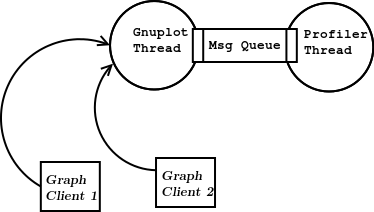
\includegraphics[width=80mm]{gnuplotthread.png}
\caption{Thread communication in between gnuplotthread and profiler thread}
\label{fig:architecture}
\end{figure}
It would be an additional advantage of having real time graph plotting when the function are executing in the background. We could able to see what are functions are currently being invoked and the relevant statistics  such as average execution time, global counters and function call frequency. Actually, embedding this features inside the VMKit would break the actual purpose of VMKit and make an extra level of overhead to upper level VM. We have overcome this issue by implementing separate thread to disseminate graph message for all gnuplot graph clients whenever they connect to VMKit. All the produced  profile messages are transmitting through the message queue channel and it will be sent over the network when client is connected to some dedicated port. Fig shows the how thread communication has performed inside the VMKit.
\section {Evaluation}

All of our experiments used identical hardware and software configurations: a single 2.4 GHz Core i3  with 4GB of memory and running a Linux 3.8.0-39-generic kernel . In order to show how well adaptive optimization perform over non adaptive mode execution, we have carried out the following evaluation.\\
Java source file has composed with several functions such as  heavy factorial calculations and matrix multiplications. 

The following graph is showing the X86-64 machine code size in two different modes which are non-optimized and optimized. After we applied several LLVM passes , optimized code has yielded highest optimized code and size of the machine code is significantly very low. When the program startup non optimized machine will be executed to reduce the initial boot up time and when the time goes fully optimized code will be patched during the runtime.
\begin{figure}[ht!]
\centering
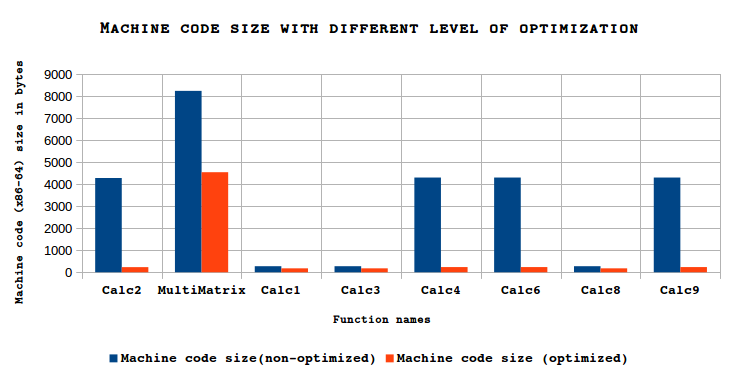
\includegraphics[width=80mm]{graph1.png}
\caption{\small Machine code size with different level of optimization}
\label{fig:machinecodesize}
\end{figure}
One of the function(Calc1) has been chosen among other functions to compare the non-adaptive and adaptive mode performance during the execution of the program. Every 20 sec interval the following calculations are being carried out.
Function call frequency – How many time particular function has been invoked in one sec
Global counter deviation -  The difference of global counters during the 20 sec time interval.
Optimized Calc1 function has replaced in the memory after 20 sec and we can clearly see the significant improvement on the rest of adaptive mode execution. Once the optimized code has  placed in to the memory the deviation of global counter and frequency  have increased. We gained this performance moderation because of the optimized code is always running after the 20 sec.
\begin{figure}[ht!]
\centering
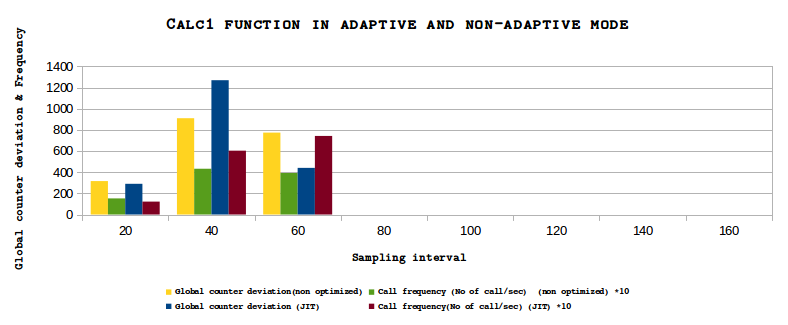
\includegraphics[width=80mm]{graph2.png}
\caption{\small Modified components in existing VMKit}
\label{fig:calc1}
\end{figure}

Another function MultiMatric which had the highest processing method among others have chosen to analysis our two type of approach.  According to our previous machine code size graph observation the size of MultiMatric has reduced to half of the size of non-optimized code, even though such a reduction is possible in the MultiMatric function,  the following graph didn't show any significant  performance improvement during the runtime. Why ? Calling frequency of this function is  comparatively very low and we couldn't able to see the 
significant improvement over non-adaptive mode of execution.
\begin{figure}[ht!]
\centering
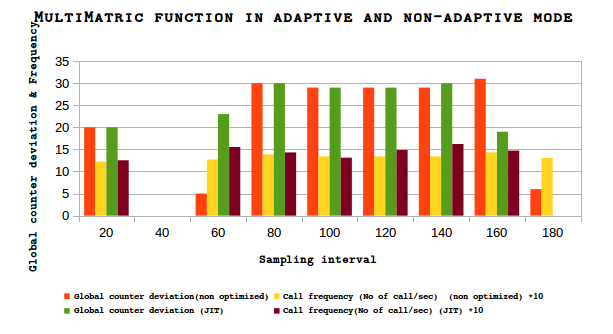
\includegraphics[width=80mm]{graph3.png}
\caption{\small Modified components in existing VMKit}
\label{fig:matrixmul}
\end{figure}

Finally we have moderated the given user input file with different loop count in order to extend the program running time so that adaptive mode of execution will take an advantage of that. The program has started with loop count 2000 and inside the loop different combinations of the functions have been called , It will give an opportunities to other function to compile with new optimized form then will be replaced in the memory.  Blue line indicates the non-adaptive mode of execution and it almost linearly grows with number of loop count mean while orange line denotes the adaptive mode of execution and it also grows with loop count but with slowest rate. If we use different level of optimization in the adaptive mode , we could able to see the wide deviation in the execution time.
\begin{figure}[ht!]
\centering
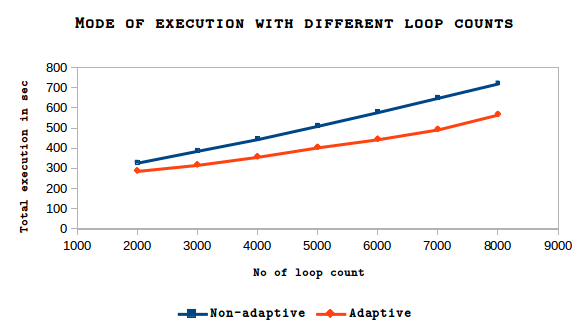
\includegraphics[width=80mm]{graph4.png}
\caption{\small Modified components in existing VMKit}
\label{fig:totalexecutiontime}
\end{figure}
